%%%%%%%%%%%%%%%%%%%%%%%%%%%%%%%%%%%%%%%%%
% Dreuw & Deselaer's Poster
% LaTeX Template
% Version 2.0 (February 18, 2023)
%
% This template originates from:
% https://www.LaTeXTemplates.com
%
% Authors:
% Vel (vel@latextemplates.com)
% Philippe Dreuw and Thomas Deselaers (https://github.com/deselaers/latex-beamerposter)
%
% License:
% CC BY-NC-SA 4.0 (https://creativecommons.org/licenses/by-nc-sa/4.0/)
%
% NOTE: The bibliography needs to be compiled using the bibtex engine.
%
%%%%%%%%%%%%%%%%%%%%%%%%%%%%%%%%%%%%%%%%%

%----------------------------------------------------------------------------------------
%	PACKAGES AND OTHER DOCUMENT CONFIGURATIONS
%----------------------------------------------------------------------------------------

\documentclass{beamer} % Use the beamer base class

\usepackage[
	orientation=portrait, % Portrait orientation
	size=a0, % Paper size
	scale=1.21, % Scale, it's important to adjust this so your content fits nicely in the template
]{beamerposter} % Use the beamerposter package to create the layout

\usetheme{I6pd2} % Use the I6pd2 theme supplied with this template

\usepackage{changepage} % Required for temporarily indenting text blocks

\usepackage{amsmath,amsthm,amssymb,latexsym} % For including math equations, theorems, symbols, etc

\usepackage{gfsdidot} % Use the GFS Didot font

\usepackage{booktabs} % Top and bottom rules for tables

\graphicspath{{Figures/}} % Location of figure images

%----------------------------------------------------------------------------------------
%	TITLE SECTION
%----------------------------------------------------------------------------------------

\title{\LARGE Volatility Forecasting Using Similarity-based Parameter Correction and Aggregated Shock Information} % Poster title

\author{David P. Lundquist\textsuperscript{1} and Daniel J. Eck\textsuperscript{1}} % Author(s)

\institute{\textsuperscript{1}Department of Statistics, University of Illinois Urbana-Champaign} % Institution(s)

%----------------------------------------------------------------------------------------
%	FOOTER TEXT
%----------------------------------------------------------------------------------------

\newcommand{\leftfoot}{https://www.LaTeXTemplates.com} % Left footer text

\newcommand{\rightfoot}{john@latextemplates.com} % Right footer text

\setbeamertemplate{footline}{} % Uncomment this line to hide the footer

%----------------------------------------------------------------------------------------

\begin{document}

\begin{frame}[t] % The whole poster is enclosed in one beamer frame, the [t] parameter aligns everything to the top

\begin{columns}[t] % Begin multi-column layout, the [t] parameter aligns each column's content to the top

\begin{column}{0.02\textwidth}\end{column} % Empty column for horizontal whitespace

\begin{column}{0.465\textwidth} % Start the first content column

%----------------------------------------------------------------------------------------
%	OBJECTIVES
%----------------------------------------------------------------------------------------

\begin{block}{Introduction}
	\begin{enumerate}
		\item Donec fringilla, velit id lobortis commodo, eros dui consectetur mi, ut interdum lorem dui sed mauris.
		\item Nulla ac nulla rhoncus est bibendum ullamcorper:
		\item Quisque vestibulum, nisl sit amet gravida ultricies dis parturient montes, nascetur ridiculus musobortis commodo, eros dui consectetur mi.
	\end{enumerate}
\end{block}

%----------------------------------------------------------------------------------------
%	INTRODUCTION
%----------------------------------------------------------------------------------------
            
\begin{block}{Setting}
	Donec fringilla, velit id lobortis commodo, eros dui consectetur mi, ut interdum lorem dui sed mauris. Duis id sem nunc, a pharetra odio. Phasellus posuere \alert{semper massa}, id bibendum ligula tristique at. Integer sit amet vulputate turpis. Sed erat lacus, faucibus at viverra et, mattis nec sem. Cras faucibus scelerisque cursus. Opet volutpat ligula.
	
	\bigskip % Vertical whitespace
	
	Duis semper lorem eget dui dignissim porttitor. \alert{Nulla facilisi.} In ullamcorper lorem quis dolor iaculis nec egestas enim ultricies. Cras ut mauris elit, ut lacinia dui. Proin in ante et libero hendrerit iaculis. Nulla eu erat a urna laoreet auctor id a turpis. Nam mollis tristique neque eu luctus. Suspendisse rutrum congue nisi sed convallis. Aenean id neque dolor.
\end{block}

%----------------------------------------------------------------------------------------
%	MATERIALS
%----------------------------------------------------------------------------------------

\begin{block}{Methodology}
	\begin{itemize}
		\item Vestibulum nisl, quis euismod velit eros in ligula.
		\begin{itemize}
			\item Cras rhoncus quam et augue convallis in elementum urna tincidunt.
		\end{itemize}
		\item Proin ut vestibulum augue.
		\begin{itemize}
			\item Donec dapibus sagittis neque eu ultrices.
		\end{itemize}
	\end{itemize}
	
	\bigskip % Vertical whitespace
	
	\begin{figure}
		\centering % Horizontally center
		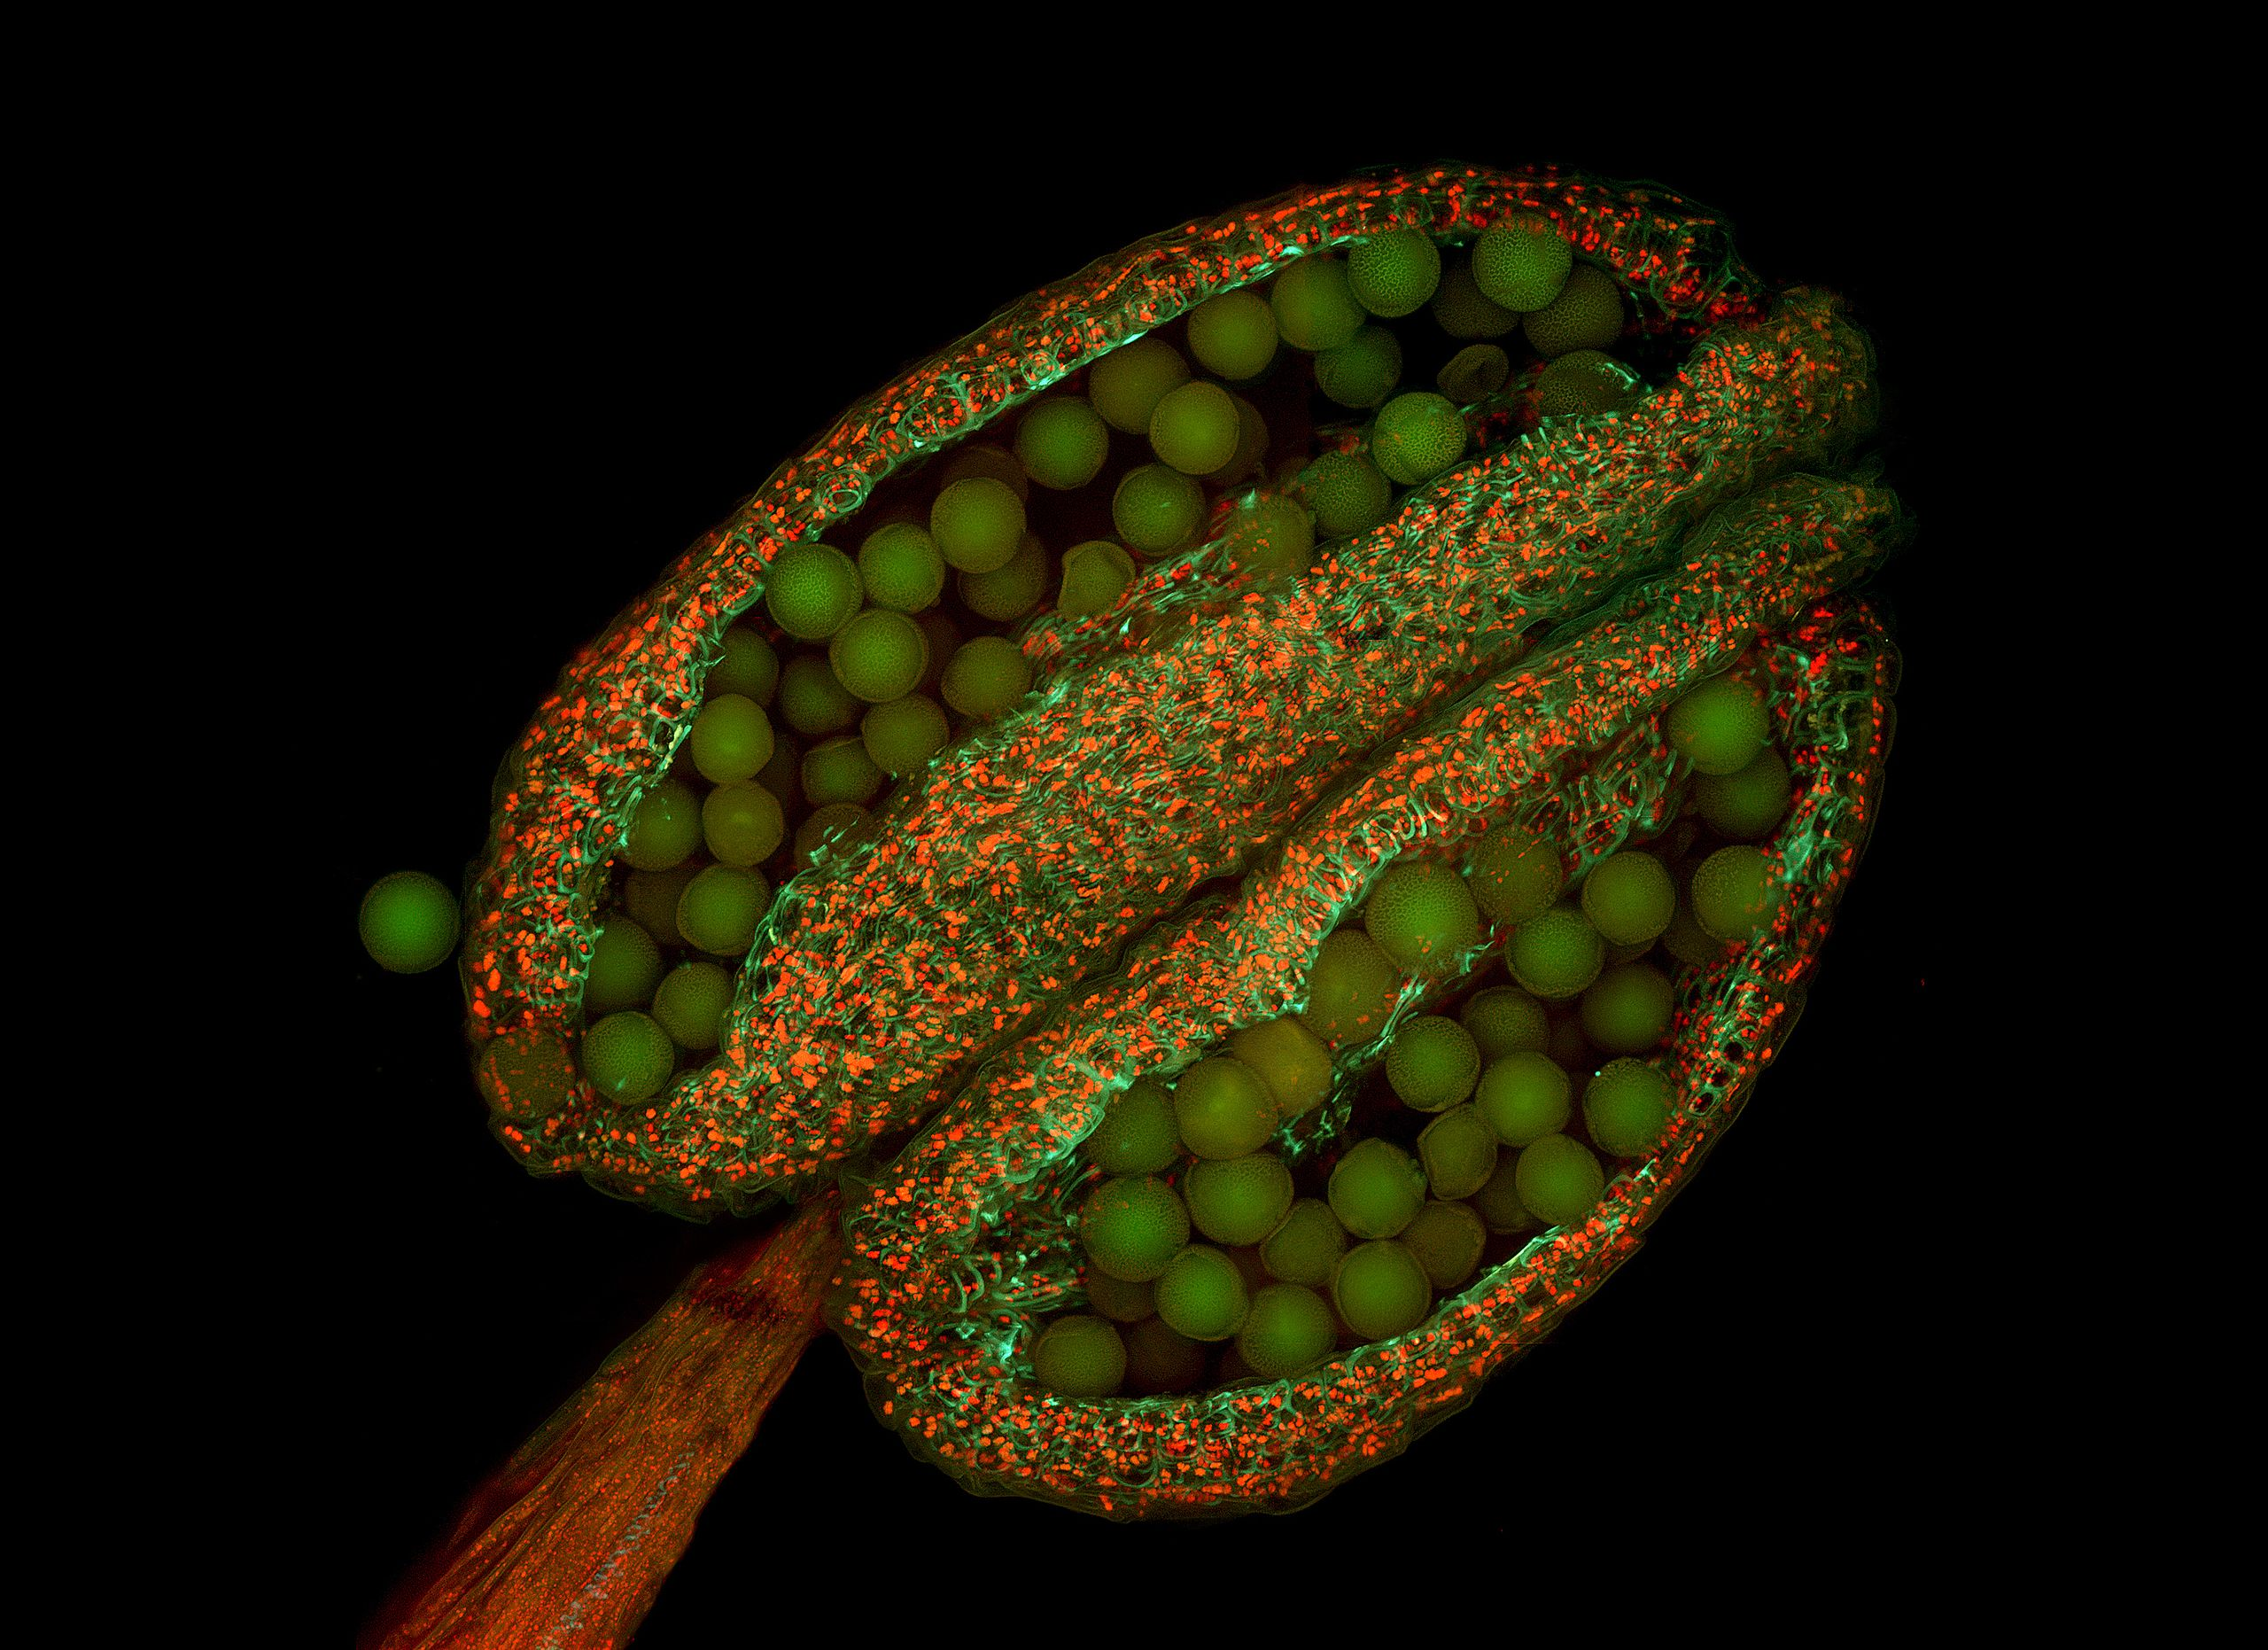
\includegraphics[width=0.65\linewidth]{Tolmukapea.jpg}
		\caption{Anther of thale cress (\textit{Arabidopsis thaliana}), fluorescence micrograph. Source: Heiti Paves, \url{https://commons.wiki-\\media.org/wiki/File:Tolmukapea.jpg}.}
	\end{figure}
\end{block}

%----------------------------------------------------------------------------------------
%	METHODS
%----------------------------------------------------------------------------------------

\begin{block}{Loss Functions}	
	\begin{itemize}
		\item International support:
		\begin{itemize}
			\item àáâäãåèéêëìíîïòóôöõøùúûüÿýñçčšž
			\item ÀÁÂÄÃÅÈÉÊËÌÍÎÏÒÓÔÖÕØÙÚÛÜŸÝÑ
			\item ßÇŒÆČŠŽ
		\end{itemize}
		\item Maecenas Vel Nisl Elit
		\begin{itemize}
			\item Suspendisse potenti. Fusce a est eget turpis rhoncus varius sed sed dui. Cras justo nibh, bibendum a cursus eget, consequat et dui. Maecenas vel nisl elit, sed dignissim dolor. 
			\item In hac habitasse platea dictumst.
		\end{itemize}
		
		\item Viewpoint Matching Constraints
		\begin{itemize}
			\item Cum sociis natoque penatibus et magnis dis parturient montes, nascetur ridiculus mus. 
			\item Proin in nisi diam.
			\item Nam ultricies pellentesque nunc, ultrices volutpat nisl ultrices a.
		\end{itemize}
	\end{itemize}
\end{block}

%----------------------------------------------------------------------------------------
%	MATHEMATICS
%----------------------------------------------------------------------------------------

\begin{block}{Properties of Volatility Shocks and Shock Estimators}
	Lorem ipsum dolor sit amet, consectetur adipiscing elit. Praesent porttitor arcu luctus, imperdiet urna iaculis, mattis eros. Pellentesque iaculis odio vel nisl ullamcorper, nec faucibus ipsum molestie. Sed dictum nisl non aliquet porttitor.
	\begin{equation}
		X \rightarrow r(X) = \arg \max_{c} \Big\{ \max_n \big\{ \sum_{x_i \in X} \delta(x_i,Y_{n,c})\big\} \Big\} 
	\end{equation}
	Etiam vulputate arcu dignissim, finibus sem et, viverra nisl. Aenean luctus congue massa, ut laoreet metus ornare in. Nunc fermentum nisi imperdiet lectus tincidunt vestibulum at ac elit. Nulla mattis nisl eu malesuada suscipit.
	\begin{equation}
		\cos^3 \theta =\frac{1}{4}\cos\theta+\frac{3}{4}\cos 3\theta
	\end{equation}
\end{block}

%----------------------------------------------------------------------------------------

\end{column} % End of the first column

\begin{column}{0.03\textwidth}\end{column} % Empty column for horizontal whitespace
 
\begin{column}{0.465\textwidth} % Start the second content column

%----------------------------------------------------------------------------------------
%	RESULTS
%----------------------------------------------------------------------------------------

\begin{block}{Numerical Examples}
	\begin{itemize}
		\item Ased Aliquet Luctus Lectus
	\end{itemize}
	
	\begin{table}
		\caption{Table caption.}
		\begin{tabular}{l l l}
			\toprule
			\textbf{Treatments} & \textbf{Response 1} & \textbf{Response 2}\\
			\midrule
			Treatment 1 & 0.0003262 & 0.562 \\
			Treatment 2 & 0.0015681 & 0.910 \\
			Treatment 3 & 0.0009271 & 0.296 \\
			\bottomrule
		\end{tabular}
	\end{table}
	
	\bigskip\bigskip % Vertical whitespace
	
	Aliquam arcu turpis, ultrices sed luctus ac, vehicula id metus. Morbi eu feugiat velit, et tempus augue. Proin ac mattis tortor. Donec tincidunt, ante rhoncus luctus semper, arcu lorem lobortis justo, nec convallis ante quam quis lectus.
	
	\begin{table} % Single column table
		\caption{Another table caption.}
		\begin{tabular}{l l r}
			\toprule
			\multicolumn{2}{c}{\textbf{Location}} \\
			\cmidrule(r){1-2}
			East Distance & West Distance & Count \\
			\midrule
			100km & 200km & 422 \\
			350km & 1000km & 1833 \\
			600km & 1200km & 890 \\
			\bottomrule
		\end{tabular}
	\end{table}
	
	\bigskip\bigskip % Vertical whitespace
	
	\begin{itemize}
		\item Vivamus lobortis eros et massa porta porttitor.
	\end{itemize}
\end{block}

%------------------------------------------------

\begin{block}{Real Data Example}
	\begin{figure}
		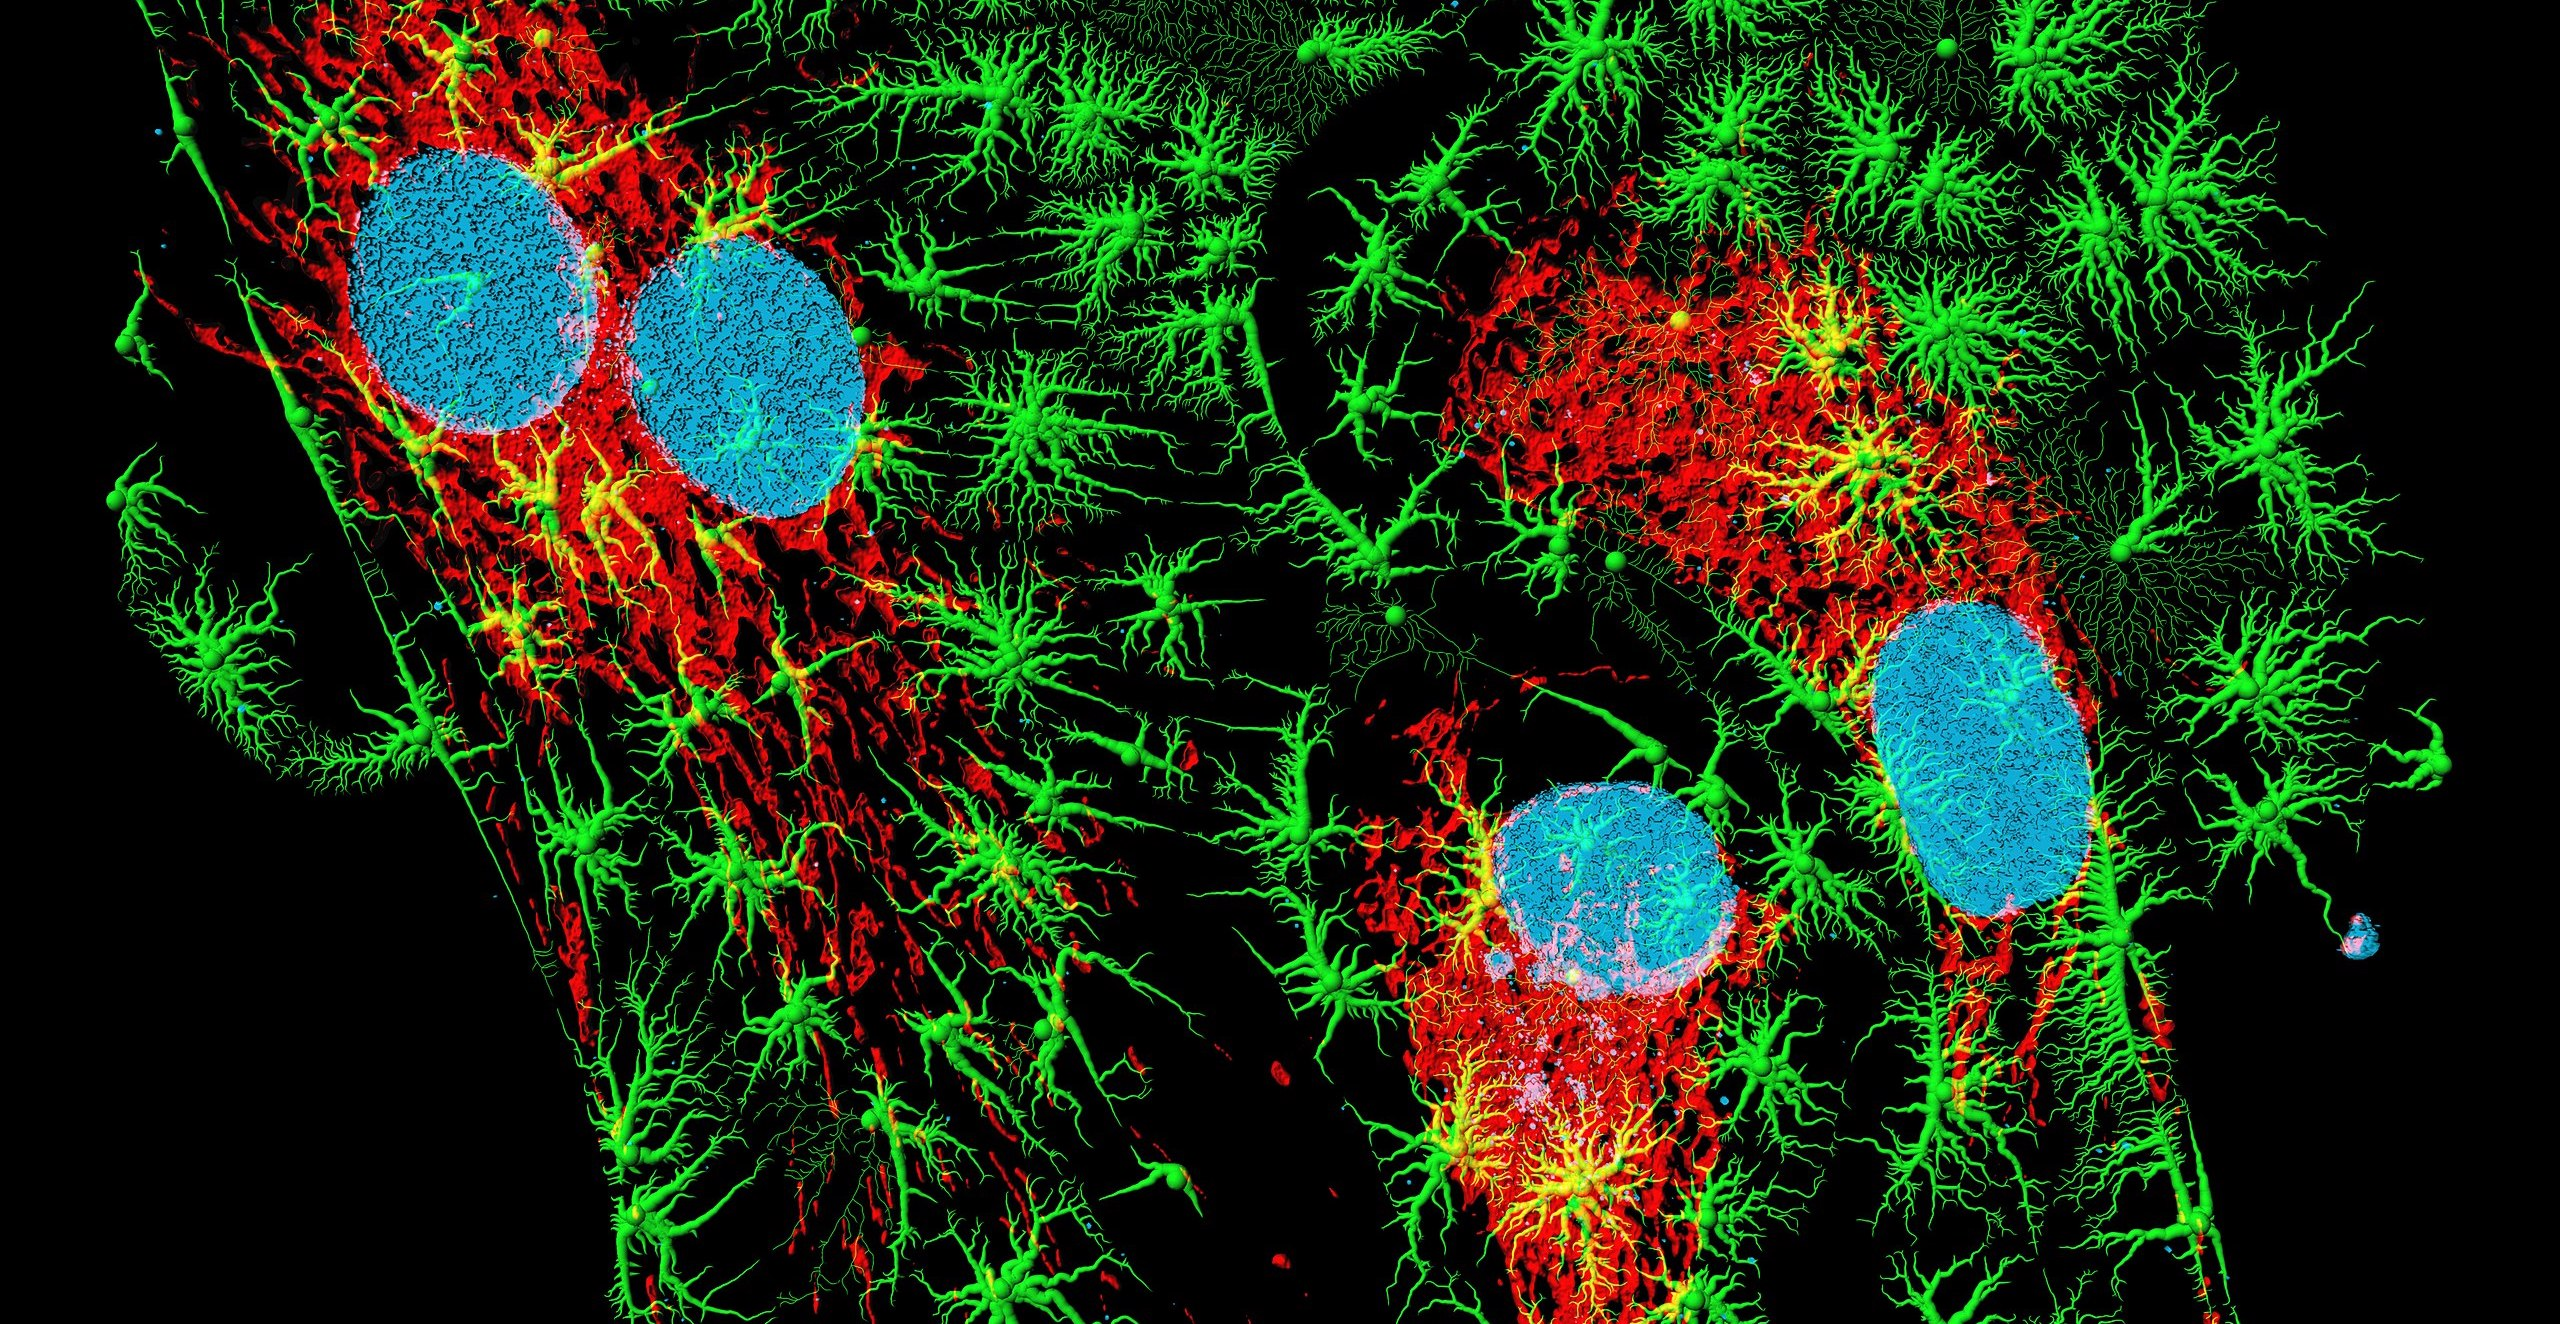
\includegraphics[width=\linewidth]{Fibroblastid.jpg}
		\caption{Bovine pulmonary artery endothelial cells in culture. Blue: nuclei; red: mitochondria; green: microfilaments. Computer generated image from a 3D model based on a confocal laser scanning microscopy using fluorescent marker dyes. Source: Heiti Paves, \url{https://commons.wikimedia.org/wiki/File:Fibroblastid.jpg}.}
	\end{figure}
\end{block}

%----------------------------------------------------------------------------------------
%	CONCLUSIONS
%----------------------------------------------------------------------------------------

\begin{block}{Conclusions}
	\begin{enumerate}
		\item \alert{Opet volutpat ligula.} Duis semper lorem eget dui dignissim porttitor. Nulla facilisi. In ullamcorper lorem quis dolor iaculis nec egestas enim ultricies. Cras ut mauris elit, ut lacinia dui. Proin in ante et libero hendrerit iaculis.
	\end{enumerate}
\end{block}

%----------------------------------------------------------------------------------------
%	REFERENCES
%----------------------------------------------------------------------------------------

\begin{block}{References}
	\nocite{*} % Insert publications even if they are not cited in the poster
	\small % Reduce font size
	\vspace{-1ex} % Pull up slightly
	\bibliographystyle{unsrt} % Bibliography style
	\bibliography{../synthVolForecast.bib} % Bibliography file
\end{block}

%----------------------------------------------------------------------------------------
%	ACKNOWLEDGEMENTS
%----------------------------------------------------------------------------------------

\begin{block}{Acknowledgements}
	\textbf{Nam mollis} tristique neque eu luctus. Suspendisse rutrum congue nisi sed convallis. Aenean id neque dolor. \textbf{Pellentesque habitant} morbi tristique senectus et netus et malesuada fames ac turpis egestas.
\end{block}

%----------------------------------------------------------------------------------------
%	CONTACT INFORMATION
%----------------------------------------------------------------------------------------

\setbeamercolor{block title}{fg=black, bg=taorange} % Change the block title color

\begin{block}{Contact Information}
	\begin{itemize}
		\item Web: \href{https://www.university.edu/labname}{https://www.university.edu/labname}
		\item Email: \href{mailto:davidl11@illinois.edu}{davidl11@illinois.edu}
	\end{itemize}
\end{block}

%----------------------------------------------------------------------------------------

\end{column} % End of the second column

\begin{column}{0.02\textwidth}\end{column} % Empty column for horizontal whitespace

\end{columns} % End of all the columns in the poster

\end{frame} % End of the enclosing frame

%----------------------------------------------------------------------------------------

\end{document}
